\documentclass[a4paper,10pt]{report}
\usepackage{amsthm}
\usepackage{amssymb}
\usepackage[centertags]{amsmath}
\edef\restoreparindent{\parindent=\the\parindent\relax}
\usepackage[parfill]{parskip}  				% Newlines create actual paragraphs
\restoreparindent
\usepackage{algorithm} 						% For pseudocode
\usepackage{algpseudocode}  					% For pseudocode
\usepackage{hyperref}						% Adds hyperlinks
\usepackage{bm}								% Bold math
\usepackage{tikz}							% Graph drawing
\usepackage{subcaption}						% Subfigures
\usepackage[toc]{appendix}					% Appendices
\usepackage{multicol}
\usepackage{color}

\usepackage[T1]{fontenc}
\usepackage[sc]{mathpazo}

\usepackage[twoside,bindingoffset=1cm]{geometry}
\usepackage{indentfirst}

% Add spacing between theorems, which is zeroed by parskip
\makeatletter
\def\thm@space@setup{%
  \thm@preskip=\parskip \thm@postskip=0pt
}
\makeatother

% Better looking empty set
\let\oldemptyset\emptyset
\let\emptyset\varnothing

% algpseudocode modifications
\renewcommand{\algorithmicrequire}{\textbf{Input:}}
\renewcommand{\algorithmicensure}{\textbf{Output:}}
\algnewcommand{\Continue}{\State \textbf{continue}}

% Theorem keyword definitions
\newtheorem{theorem}{Theorem}[chapter]
\newtheorem{definition}[theorem]{Definition}
\newtheorem{proposition}[theorem]{Proposition}
\newtheorem{lemma}[theorem]{Lemma}
\newtheorem{corollary}[theorem]{Corollary}

% DEBUG commands
\newcommand{\DEBUGComment}[1]{{\color{red}{#1}}}
\newcommand{\DEBUGQuestion}[1]{{\color{blue}{#1}}}

\usepackage{fancyhdr}
\pagestyle{fancy}
\renewcommand{\chaptermark}[1]{\markboth{#1}{}}
\renewcommand{\sectionmark}[1]{\markright{\thesection\ #1}}
\fancyhf{} \fancyhead[LE,RO]{\bfseries\thepage}
\fancyhead[LO]{\bfseries\rightmark} \fancyhead[RE]{\bfseries\leftmark}


%%%%%%%%%%%%%%%%%%%%%%%%%%%%%%%%%%%%%%

\begin{document}

\pagestyle{empty}

%%% Title
\begin{titlepage}
\begin{center}
\begin{figure}[htb]
\begin{center}

\includegraphics[width=6cm]{ub.png}
\end{center}
\end{figure}

\textbf{\LARGE Treball final de grau} \\
\vspace*{.5cm}
\textbf{\LARGE GRAU DE MATEMÀTIQUES } \\
\vspace*{.5cm}
\textbf{\LARGE Facultat de Matemàtiques i Informàtica \\ Universitat de Barcelona} \\
\vspace*{1.5cm}
\rule{16cm}{0.1mm}\\
\begin{Huge}
\textbf{PATHFINDING ALGORITHMS IN GRAPHS AND APPLICATIONS} \\
\end{Huge}
\rule{16cm}{0.1mm}\\

\vspace{1cm}

\begin{flushright}
\textbf{\LARGE Autor: Daniel Monzonís Laparra}

\vspace*{2cm}

\renewcommand{\arraystretch}{1.5}
\begin{tabular}{ll}
\textbf{\Large Director:} & \textbf{\Large Dr. Antoni Benseny} \\
\textbf{\Large Realitzat a:} & \textbf{\Large  Departament de Matemàtica Aplicada i Anàlisi} \\
\\
\textbf{\Large Barcelona,} & \textbf{\Large \today }
\end{tabular}

\end{flushright}
\end{center}
\end{titlepage}


\section*{Abstract}
The aim of this work is to give a rigorous mathematical insight of the most popular pathfinding algorithms, focusing on $A^*$ and trying to understand how the heuristic it uses affects its correctness and performance. We complement this theoretical study of the algorithms with experimental results found by running two benchmarks of the algorithms.
{\let\thefootnote\relax\footnote{2010 Mathematics Subject Classification. 05C12, 05C38, 05C85, 68R10}}


\tableofcontents

\pagestyle{fancy}
\chapter{Introduction}
Many problems in the fields of science, mathematics and engineering can be generalised to the problem of finding a path in a graph. Examples of such problems include routing of telephone or Internet traffic, layout of printed circuit boards, automated theorem proving, GPS routing, decision making in artificial intelligence and robotics \cite{ai}.

A graph is simply a set of nodes connected to each other by edges. Depending on the problem, it can make sense to associate a number with each edge, usually called the weight of the edge. For example, in a geographical map, nodes could represent cities and towns, and the edges could represent the roads that connect them, with the weights being the total distance of each road. Then, one could ask what is the best way to travel from one city to another, that is, the set of roads that one would have to follow so that the total distance travelled is minimal with respect to all the other possible ways to get from that city to the other. One could use a brute force algorithm by finding all the possible combinations of roads that start and end at the desired cities and selecting the one with minimal distance, but as the number of nodes and edges grows larger, the number of combinations would grow extremely large and eventually we would run out of memory or the execution may take too long. That is where more sophisticated pathfinding algorithms, like the ones presented in this work, come in.

For this project, we built a pathfinding simulator which implements all the algorithms presented in the work. For the graphical part of the simulator, which will also be used to provide some example images, we use a grid graph, represented by a tiled 2D map, in which each tile or node is connected to its adjacent tiles. In the map, each tile can have a different weight, or be a wall, which is impassable. This notion of weighted nodes and walls can be translated to the structure of a weighted directed graph by thinking of the weights of the tiles as the weights of the edges that connect adjacent tiles to it. Walls can be thought of as nodes that are not connected to any other node, or that just do not exist, and therefore are not reachable from other nodes. However, the algorithms implemented are general enough to work with any other graph specification, and we will also use them with a graph generated from the roads in Florida for one of the benchmarks in the experimental part.

In Chapter 2, we provide the mathematical background and definitions we will be using throughout the entire work. Then, we present the main algorithm we will focus on, $A^*$, building up to it by first discussing other algorithms which are key to understanding how it works, since it will borrow some ideas from them. We will also prove how under certain conditions, the algorithm always finds optimal paths between any two points.

In Chapter 3 we go into detail on the main thing that makes $A^*$ special, which is the use of a heuristic function. We will see different results regarding heuristics, and see that for heuristics which satisfy a certain condition, the algorithm becomes much more efficient. In this chapter we also define some heuristics for grid graphs which work well in different situations.

Chapter 4 is a short chapter where we describe, from a user standpoint, the simulator that was developed, briefly explaining its options and functionality.

Finally, on Chapter 5, we discuss the experimental part of this work. We explain in detail the benchmarks that were performed, and present its results.


\chapter{The $A^*$ algorithm}
\label{chapter:algorithms}
The $A^*$ algorithm is a very popular algorithm used in many applications to find optimal paths between points. The algorithm works on graphs, a structure well studied in graph theory.

\begin{definition}
A \textbf{directed graph} $G$ is a pair of sets $(V, E)$, where $V$ is the set of vertices or nodes, and $E$ the set of edges, formed by pairs of vertices.
\end{definition}

\begin{definition}
A \textbf{weighted directed graph} is a graph in which $\forall e \in E \ \exists w(e) \in \mathbb{R}$. We call $w(e)$ the \textbf{weight} or \textbf{cost} of the edge $e$.

If $e = (u, v)$ for some $u, v \in V$, then we equivalently call $d(u, v) = w(e)$ the \textbf{distance} from $u$ to $v$.
\end{definition}

From now on, when we talk about a graph, we will implicitly refer to a finite weighted directed graph, since it is the most general type of graph we will work with. An unweighted graph can be thought of as a weighted graph where all weights are equal to one, and an undirected graph as a directed graph where $\forall (u, v) \in E,\  \exists (v, u) \in E$. Also, the graphs we will work with are finite, meaning that $|V| < \infty$ and $|E| < \infty$.

\begin{definition}[Path]
Given a graph $G$, and $u, v \in V$, a \textbf{path} $P$ between $u$ and $v$ is an ordered list of a certain amount of edges, $N$, in the form

\[ P = \{(u,v_1), (v_1, v_2), \dots, (v_{N-2}, v_{N-1}), (v_{N-1}, v)\} \]
\end{definition}

Note that paths are not unique. There may exist multiple paths between two nodes.

\begin{definition}
We say that two nodes $u, v \in V$ are connected $\Longleftrightarrow$ There exists a path $P$ between $u$ and $v$.
\end{definition}

\begin{definition}
Given a path $P$ between two nodes $u, v \in V$, given a node $n$ which is in the path, we say that $n'$ is the \textbf{successor} of $n$ if $(n, n') \in P$, that is, if we followed the path $P$, the next node we would visit when we have reached $n$ would be $n'$.
\end{definition}

\begin{definition}
If $u \in V$, we define the \textbf{connected component} of $u$ as
\[ C_u = \{ v \in V\ |\ u \ \text{and} \ v \ \text{are connected}\  \} \]
which is a subgraph of $G$.
\end{definition}

\begin{definition}[Distance of a path]
Given a path $P$ in a weighted directed graph $G$, we define the \textbf{weight} or \textbf{distance} of the path, $dist(P)$, as

\[ d(P) = \sum_{e \in P} w(e) \]

If $P$ is a path between $u$ and $v$, we can equivalently write

\[ d_P(u, v) = d(P) \]

If the context is clear, we will just write $d(u, v)$. For convenience, if $u$ and $v$ are not connected, we define the distance between them as $d(u, v) = \infty$.
\end{definition}

Note that, in general, $d(u, v) \neq d(v, u)$, since graphs can be directed and not all paths may be reversible.

\begin{definition}[Optimal path]
\label{def:optimal}
Given a set of all the existing paths between two nodes $u$ and $v$, $\chi_{(u, v)}$, we will say that a path $P \in \chi_{(u,v)}$ is \textbf{optimal} if and only if $d(P) \le d(P') \ \forall P' \in \chi_{(u, v)}$.
\end{definition}

We will also say that $P$ is the \textbf{shortest distance path} if it is optimal, and we will write the distance that fulfils the condition in definition \ref{def:optimal} as $\delta(u,v)$. Clearly, in a finite graph, an optimal path between any two nodes always exists, since in this case $\chi_{(u, v)}$ is finite.

Instead of presenting the $A^*$ algorithm without any background, we will first briefly discuss some other widely known algorithms that can be used to find paths between nodes in graphs, and build up to the main algorithm by trying to gradually improve the performance.

\section{BFS}
Breadth-First Search, or BFS for short, attempts to find a path by methodically examining all the neighbours of each node it examines.

The algorithm uses a queue\footnote{See \ref{annex:queue} for more information on queues.} to keep track of the next nodes to examine, adding all unvisited neighbours of a node when it is examined, until the queue is empty. Explored nodes are kept in a set, so that we don't explore the same node twice. The set of nodes that haven't been explored yet is often called the \emph{open set}, and the set of visited nodes the \emph{closed set}. In the same way, nodes in the open set are called \emph{open nodes}, and nodes in the closed set are called \emph{closed nodes}.

The pseudocode for the algorithm is presented in algorithm \ref{alg:bfs}. The algorithm returns a map called \emph{previous}, which maps every node to the node we came from in the path that the algorithm computes. The procedure that we will use to reconstruct the path from this map for all algorithms is presented in algorithm \ref{alg:reconstruct}.

\begin{algorithm}
\caption{Breadth-First Search}
\label{alg:bfs}
\begin{algorithmic}[1]
\Procedure{BFS}{$G, \alpha, \beta$}
\Require Graph $G = (V, E)$, directed or undirected; source node $\alpha \in V$; goal node $\beta \in V$
\Ensure Given $u \in V$, previous[$u$] gives us the node come from to reach $u$ in the path computed
\State Q $\gets Queue()$
\State $S \gets Set()$ \Comment{Keeps track of explored nodes}
\State previous $\gets Map()$
\For {$u \in V$}
	\State previous[$u$] $\gets \varnothing$
\EndFor
\State Q.enqueue($\alpha$)
\State $S$.add($\alpha$)
\While {not Q.empty()}
	\State $u \gets$ Q.front()
	\State Q.dequeue()
	\For {v $\in$ $u$.neighbours()}
		\If {$v \not\in S$}
			\State Q.enqueue($v$)
			\State S.add($v$)
			\State previous[$v$] $\gets u$
		\EndIf
	\EndFor
\EndWhile
\State \Return ReconstructPath(previous, $\alpha$, $\beta$)
\EndProcedure
\end{algorithmic}
\end{algorithm}

\begin{algorithm}
\caption{Reconstruct path}
\label{alg:reconstruct}
\begin{algorithmic}[1]
\Procedure{ReconstructPath}{previous, $\alpha$, $\beta$}
\Require The map $previous$ returned by the pathfinding algorithm; source node $\alpha \in V$; goal node $\beta \in V$
\Ensure An ordered list $P$ with the nodes from the path from $\alpha$ to $\beta$
\State $P \gets$ []  \Comment{Empty array for the path}
\State $u \gets \beta$
\While {$u \neq \alpha$}
	\State $P$.push($u$)
	\State $u \gets$ previous[$\beta$]
\EndWhile
\State $P$.push($\alpha$)
\State \Return $P$.reversed()
\EndProcedure
\end{algorithmic}
\end{algorithm}

In the rest of this work, we will consider a set of goal nodes instead of a single goal node, since this makes the algorithms, and therefore the results shown, more general. We will call this set of goal nodes $T$. This way, having a single goal node is only a special case of the more general condition when $|T| = 1$.

We see that with this version of BFS, all nodes in the connected component of the starting node are explored. We can improve the performance if we halt the execution once we reach a goal node, which is a fair condition since all we're looking for is a path between the source and a goal node, and once we find it we don't need to keep searching. This new version of the algorithm with the early exit is shown in algorithm \ref{alg:bfs_early_exit}.

\begin{algorithm}
\caption{Breadth-First Search with early exit}
\label{alg:bfs_early_exit}
\begin{algorithmic}[1]
\Procedure{BFS}{$G, \alpha, T$}
\Require Graph $G = (V, E)$, directed or undirected; source node $\alpha \in V$; set of goal nodes $T \subset V$
\Ensure Given $u \in V$, previous[$u$] gives us the node come from to reach $u$ in the path computed, if it has been explored
\State Q $\gets Queue()$
\State $S \gets Set()$
\State previous $\gets Map()$
\For {$u \in V$}
	\State previous[$u$] $\gets \varnothing$
\EndFor
\State Q.enqueue($\alpha$)
\State $S$.add($\alpha$)
\While {not Q.empty()}
	\State $u \gets$ Q.front()
	\State Q.dequeue()
	\For {$v \in$ u.neighbours()}
		\If {$v \not\in$ S}
			\If {$v \in T$} \Comment{Early exit condition}
				\State \Return ReconstructPath(previous,$\alpha$,$v$)
			\EndIf
			\State Q.enqueue($v$)
			\State S.add($v$)
			\State previous[$v$] $\gets u$
		\EndIf
	\EndFor
\EndWhile
\EndProcedure
\end{algorithmic}
\end{algorithm}

Note that, even though BFS will always find a path between two nodes if they are connected, the path produced is not optimal when we consider weights. The path found will be the shortest in terms of the number of steps, but when taking into account the weights of the edges, this algorithm will not give us the shortest distance path, as we can see in figure \ref{fig:bfs-fail}.

\begin{figure}
\centering
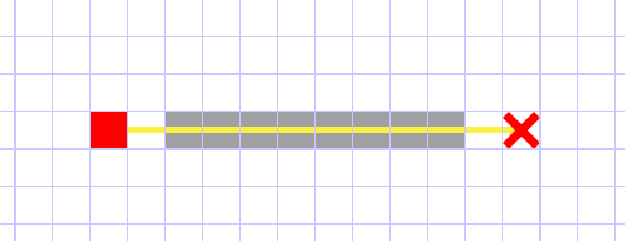
\includegraphics[width=1\linewidth]{bfs-fail}
\caption{An example on how BFS fails to find an optimal path when we use a weighted graph. In this example, moving to a white tile has cost 1, while moving to a gray tile has cost 10, so clearly, going in a straight line is not the optimal path.}
\label{fig:bfs-fail}
\end{figure}

Also, the algorithm does not seem very efficient, since we can potentially explore lots of nodes on a very dense graph.

We will first address the optimality problem in the next section, and then we will focus on efficiency.


\section{Dijkstra}
Dijkstra's algorithm \cite{dijkstra} is also a well known graph theory algorithm, used to find optimal paths between nodes in a graph with positive weights. Now, instead of a simple queue, we use a priority queue\footnote{See \ref{annex:priorityqueue} for more information on priority queues.}. We keep exploring all unvisited neighbours of a node, but now we insert them in the priority queue using the distance of the edge, in a way that the node with the least distance from the source will be extracted first.

Normally, the algorithm only gets a starting node, and computes the optimal paths to all reachable nodes from the origin, but since we're only concerned about finding the path to one of the goal nodes, we will use the early exit condition to end the execution as soon as we expand a goal node. Later, we will see that this still gives us the optimal path.

\begin{algorithm}
\caption{Dijkstra's algorithm}
\label{alg:dijkstra}
\begin{algorithmic}[1]
\Procedure{Dijkstra}{$G$, $\alpha$, $T$}
\Require Graph $G = (V, E)$, directed or undirected; source node $\alpha \in V$; set of goal nodes $T \subset V$
\Ensure Given $u \in V$, previous[$u$] gives us the node come from to reach $u$ in the path computed, and d[$u$] gives us the distance to that node, if it has been explored
\State Q $\gets PriorityQueue()$
\State $S \gets Set()$
\State d $\gets Map()$ \Comment{Keeps track of the shortest distance to each node}
\State previous $\gets Map()$
\For {$u \in V$}
	\State d[$u$] $\gets \infty$
	\State previous[$u$] $\gets \varnothing$
\EndFor
\State Q.insert((0, $\alpha$))
\State d[$\alpha$] $\gets 0$
\While {not Q.empty()}
	\State u $\gets$ Q.removeMin()
	\State S.add(u)
	\If {$u \in T$} \Comment{Early exit condition}
		\State \Return ReconstructPath(previous,$\alpha$,$u$)
	\EndIf
	\For {$v \in$ $u$.neighbours()}
		\If {$v \in S$}
			\Continue \Comment{Already explored node}
		\EndIf
		\State alt $\gets$ d[$u$] $+ w((u, v))$
		\If {alt $<$ d[$v$]}
			\State d[$v$] $\gets$ alt
			\State Q.insert(($v$, alt))
			\State previous[$v$] $\gets u$
		\EndIf
	\EndFor
\EndWhile
\EndProcedure
\end{algorithmic}
\end{algorithm}

We will now prove the correctness of the algorithm without the early exit condition, that is, given a node $u \in V$, the algorithm always finds the optimal path between $u$ and all other nodes $v \in V$ such that $u$ and $v$ are connected. We will do so by induction on the visited set used in algorithm \ref{alg:dijkstra}, $S$. We will also write the distance computed by Dijkstra's algorithm between two nodes $u, v$ as $d_D(u, v)$.

\begin{lemma}
\label{lemma:dijkstra}
At any given step of the algorithm, $\forall s \in S,\ d_D(u, s) = \delta(u, s)$
\end{lemma}
\begin{proof}
If $|S| = 0$, the statement is trivially true.

If $|S| = 1$, it must be $S = \{u\}$, since $S$ only grows in size, but $d_D(u, u) = 0 = \delta(u, u)$.

Now let's assume we are in an arbitrary step, and let $s$ be the current node being explored, not yet added to $S$. Let $S' = S \cup \{s\}$. By inductive hypothesis, we know that $\forall t \in S,\ d_D(u, t) = \delta(u, t)$. Now we only need to show that $d_D(u, s) = \delta(u, s)$.

Suppose that there exists a path $Q$ from $u$ to $s$ such that
\[d(Q) < d_D(u, s)\]
We know that the path $Q$ starts in $S$ (since $u \in S$), but at some point has to leave $S$ (since $s \not\in S$). Let $e = (x, y) \in Q \subset E$ be the first edge that leaves $S$, that is, $x \in S$ but $y \not\in S$. Let $Q_x \subset Q$ be the edges of $Q$ up until and without including the edge $e$. Clearly,
\[d(Q_x) + d(x, y) \le d(Q)\]

By the induction hypothesis, $d_D(u, x) = \delta(u, x) \le d(Q_x)$. Therefore,
\[ d_D(u, x) + d(x, y) \le d(Q) \]

Clearly, $\delta(u, y) \le d_D(u, x) + d(x, y)$.

Since $y \not\in S$, and since Dijkstra uses a priority queue to select the next reachable node with minimum distance, we know that $d_D(u, s) \le d_D(u, y)$.

Combining the inequalities, we get that
\[ d_D(u, s) \le d_D(u, y) \le d_D(u, x) + d(x, y) \le d(Q) < d_D(u, s) \]
which is a contradiction.

Therefore, $d_D(u, s) = \delta(u, s)$.
\end{proof}

\begin{theorem}[Correctness of Dijkstra's algorithm]
\label{thm:dijkstra}
Let $G = (V, E)$ be a weighted directed graph. Let $u \in V$. Then, after running Dijkstra's algorithm with start node $u$, the following is true
\[ \forall v \in C_u,\  d_D(u, v) = \delta(u, v) \]
\end{theorem}
\begin{proof}
We know that, at the end of Dijkstra's algorithm, we'll have explored all the nodes connected to $u$. That is, $S = C_u$. For each $v \in C_u$, apply \ref{lemma:dijkstra} to get the wanted result.
\end{proof}

\begin{corollary}
Given a source node and a single goal node, Dijkstra's algorithm always finds an optimal path between the two nodes if it exists.
\end{corollary}
\begin{proof}
Let $G = (V, E)$, and let $\alpha, \beta \in V$ be the source and goal nodes, respectively. If $\beta \not \in C_\alpha$, an optimal path does not exist. Suppose $\beta \in C_\alpha$. By Theorem \ref{thm:dijkstra}, after running Dijkstra, $d_D(\alpha, \beta) = \delta(\alpha, \beta)$, so an optimal path has been found.
\end{proof}

Like with BFS, we can modify the algorithm to use early exit to improve performance.
\begin{proposition}
Using Dijkstra's algorithm with early exit with start node $\alpha$ and a single goal node $\beta$ ensures that an optimal path from $\alpha$ to $\beta$ will be found.
\end{proposition}
\begin{proof}
With early exit, when we explore the goal node $\beta$ we will end the execution of the algorithm. Using \ref{lemma:dijkstra}, we know that $d_D(u, \beta) = \delta(u, \beta)$, so we already have the optimal path between the two nodes.
\end{proof}

Note that Dijkstra's algorithm only works for graphs with positive weights. In graphs with negative weights, it could possibly get stuck in an infinite loop of negative weight edges, since the total cost can become smaller indefinitely. For graphs with negative weights, there are other algorithms to find optimal paths, albeit significantly less efficient, like the Bellman-Ford algorithm \cite{bellman-ford}.

\section{Greedy Best-First search}
\label{section:greedy}
As we have seen in the last section, we now have an algorithm that can find the optimal path between any two nodes in a graph with positive weights. We will now start to worry about improving the performance of the algorithm.

\begin{definition}
Given any node $u \in V$, $t \in T$ is a \textbf{preferred goal node} of $u$ if the distance of an optimal path from $u$ to $t$ does not exceed the distance of any other path from $u$ to a node in $T$.
\end{definition}

Let's forget about optimality for a moment, and modify our pathfinding algorithm to use only a heuristic. A heuristic is a function
\begin{align*}
	h \colon V &\to \mathbb{R}\\
	u &\mapsto h(u)
\end{align*}
which gives an estimate of the distance from a node to one of its preferred goal nodes, which we compute without having to expand extra nodes, and varies with each type of problem we have.

We will talk more about heuristics later, but for now, let's consider what happens when we use heuristics instead of the actual distance of the paths between nodes, like we did in Dijkstra's algorithm, for the priority queue ordering. When using the heuristic as ordering, the node closest to the goal will be the first to be explored, not regarding the distance travelled so far.

\begin{algorithm}
\caption{Greedy Best-First search}
\label{alg:greedy}
\begin{algorithmic}[1]
\Procedure{GreedyBestFirstSearch}{$G$, $\alpha$, $T$}
\Require Graph $G = (V, E)$, directed or undirected; source node $\alpha \in V$; set of goal nodes $T \subset V$
\Ensure Given $u \in V$, previous[$u$] gives us the node come from to reach $u$ in the path computed, if it has been explored
\State Q $\gets PriorityQueue()$
\State $S \gets Set()$
\State previous $\gets Map()$
\For {$u \in V$}
	\State previous[$u$] $\gets \varnothing$
\EndFor
\State Q.insert((0, $\alpha$))
\While {not Q.empty()}
	\State $u \gets$ queue.removeMin()
	\State S.add($u$)
	\If {$u \in T$} \Comment{Early exit condition}
		\State \Return ReconstructPath(previous,$\alpha$,$u$)
	\EndIf
	\For {$v \in$ $u$.neighbours()}
		\If {$v \in S$}
			\Continue
		\EndIf
		\State Q.insert(($v$, $h(v)$))
		\State previous[$v$] $\gets u$
	\EndFor
\EndWhile
\EndProcedure
\end{algorithmic}
\end{algorithm}

As we will see later in this work, this algorithm tends to finish much faster than Dijkstra. However, it does not produce optimal paths in general, since all it uses is the heuristic, so no information from the actual costs is used at all.

\section{$A^*$}
\label{section:astar}
As we have seen, Dijkstra always gives us optimal paths, but it wastes a lot of time exploring a lot of nodes that are not in a promising direction. On the other hand, Greedy Best-First Search explores nodes in a promising direction, but does not produce optimal paths reliably.

The $A^*$ algorithm is a combination of both algorithms. It takes into account both the actual distance from the source to a node, and the estimated distance from the node to the goal. Unlike Dijkstra's algorithm, which works for positive weights including zero, $A^*$ only works with strictly positive weights. It was first described in 1968 by Peter Hart, Nils Nilsson and Bertram Raphael \cite{hart}.

\begin{definition}
If an algorithm $A$ always finds an optimal path between the source node and a preferred goal node, we say that $A$ is \textbf{admissible}.
\end{definition}

Given a source node $\alpha \in V$ and a set of goal nodes $T$, let $\hat{f}(u) = \hat{g}(u) + \hat{h}(u)$, where 
\begin{align*}
\hat{g}(u) = \delta(\alpha, u)\\
\hat{h}(u) = \min_{t \in T} \delta(u, t)
\end{align*}
 
Note that for any node $v$ in an optimal path between $\alpha$ and a preferred goal node $t$ of $\alpha$, $\hat{f}(v) = \hat{f}(\alpha) = \hat{f}(t) = \delta(\alpha, t)$. We will usually write this distance as $f^*$.

Let $g(u)$ and $h(u)$ be functions which give us estimates for $\hat{g}(u)$ and $\hat{h}(u)$ respectively.

\begin{definition}
Given a source node and a set of goal nodes in a graph $G = (V, E)$, we define the \textbf{score} as a function $f \colon V \to \mathbb{R}$ defined as
\begin{equation}
	f(u) = g(u) + h(u)
\end{equation}
where $g(u)$ is an estimate of the optimal distance from the source to the node $u$, and $h(u)$ is an estimate of the optimal distance from the node $u$ to one of its preferred goal nodes. We usually call $g$ the \textbf{g-score}, and $h$ the \textbf{h-score}.
\end{definition}

In $A^*$, a good choice for the g-score is using, for each node $u$, the cost of the path from the source to $u$ found so far by the algorithm, which is equivalent to the distance we kept updating in Dijkstra's algorithm. Note that this implies $g(u) \geq \hat{g}(u) \ \forall u \in V$. For the h-score, we use some heuristic, which will depend on the problem.

When a node is explored, its g-score, and thus its score will be updated. The pseudocode for the algorithm is shown in algorithm \ref{alg:astar}. As we can see, it is very similar to Dijkstra's, except that we now use the score for the priority queue ordering, instead of just the distance to that node.

\begin{algorithm}
\caption{$A^*$ algorithm}
\label{alg:astar}
\begin{algorithmic}[1]
\Procedure{AStar}{$G$, $\alpha$, $T$}
\Require Graph $G = (V, E)$, directed or undirected; source node $\alpha \in V$; set of goal nodes $T \subset V$
\Ensure Given $u \in V$, previous[$u$] gives us the node come from to reach $u$ in the path computed, and g[$u$] is the current g-score of the node
\State Q $\gets PriorityQueue()$
\State $S \gets Set()$
\State $g \gets Map()$
\State previous $\gets Map()$
\For {$u \in V$}
	\State g[$u$] $\gets \infty$
	\State previous[$u$] $\gets \varnothing$
\EndFor
\State Q.insert((0, $\alpha$))
\State $g[\alpha]$ $\gets 0$
\While {not Q.empty()}
	\State $u \gets$ Q.removeMin()
	\State $S$.add($u$)
	\If {$u \in T$} \Comment{Early exit condition}
		\State \Return ReconstructPath(previous,$\alpha$,$u$)
	\EndIf
	\For {$v \in u$.neighbours()}
		\State alt $\gets g[u] + w((u, v))$
		\If {alt $< g[v]$}
			\State $g[v] \gets$ alt \Comment{Update the g-score}
			\State $f = g[v] + h(v)$
			\State Q.insert(($v$, $f$))
			\State previous[$v$] $\gets u$
		\EndIf
	\EndFor
\EndWhile
\EndProcedure
\end{algorithmic}
\end{algorithm}

This new algorithm is faster than Dijkstra, but it only finds optimal reliably paths under a certain condition, which is what we will prove next.

\begin{definition}
A heuristic $h$ is said to be \textbf{admissible} if and only if, $\forall u \in V$, $h(u)$ never overestimates the real cost of moving from $u$ to a preferred goal node of $u$, that is, 
\[ \forall u \in V \ h(u) \le \hat{h}(u) \]
\end{definition}

We will prove that, with the score function we have constructed, an admissible heuristic implies that $A^*$ is admissible. Consider a graph $G = (V, E)$, a source node $\alpha$ and a set of goal nodes $T$, such that $\forall t \in T$, $t \in C_\alpha$. Consider the closed set $S$, which corresponds to the set of visited nodes in the algorithm, and the open set $O$, which are the nodes that haven't been explored yet.

\begin{lemma}
\label{lemma:astar1}
For any node $u \not \in S$ and for any optimal path $P$ from $\alpha$ to $u$, $\exists v \in O$ which is part of $P$ such that $g(v) = \hat{g}(v)$.
\end{lemma}
\begin{proof}
Consider an optimal path from $\alpha$ to $u$,
\[P = \{ (u_0 = \alpha, u_1), (u_1, u_2), \dots, (u_{n-1}, u_n = u) \}\]

If $v = \alpha$, which implies that $\alpha \in O$, so the algorithm hasn't completed the first iteration yet, then the lemma is trivially true since $g(\alpha) = \hat{g}(\alpha) = 0$.

Now suppose $\alpha \in S$. Let
\[ \Delta = \{ n \in S \  | \  n \text{ is part of } P,\  g(n) = \hat{g}(n) \} \]
$\Delta$ is clearly not empty since $\alpha \in \Delta$.

Let $n^* \in \Delta$ be the node that satisfies $d_P(\alpha, n^*) \leq d_P(\alpha, n) \  \forall n \in \Delta$. Since $w(e) > 0\  \forall e \in E$, $n^*$ is unique. Also, $n^* \neq u$ since $u \not \in S$. Let $v$ be the successor of $n^*$ in $P$. Note that it is possible that $v = u$.

Now, $g(v) \leq g(n^*) + w((n^*, v))$ by the definition of $g$, and since $n^* \in \Delta$, $g(n^*) = \hat{g}(n^*)$. Also, $\hat{g}(v) = \hat{g}(n^*) + w((n^*, v))$, because $P$ is an optimal path. Therefore, $g(v) \leq \hat{g}(v)$. But it is always true that $g(v) \geq \hat{g}(v)$. Therefore, $g(v) = \hat{g}(v)$, and by the definition of $\Delta$, $v \not \in \Delta$ implies $v \in O$.
\end{proof}

\begin{lemma}
\label{lemma:astar2}
Suppose the heuristic used by $A^*$ is admissible, and suppose $A^*$ has not finished its execution yet. Then, for any optimal path $P$ from $\alpha$ to a preferred goal node of $\alpha$, $\exists v \in O$ which is part of $P$ such that $f(v) \leq f^*$.
\end{lemma}
\begin{proof}
By lemma \ref{lemma:astar1}, $\exists v$ in $P$ with $g(v) = \hat{g}(v)$. Therefore, by the definition of the score function and the hypothesis,
\begin{align*}
f(v) &= g(v) + h(v)\\
&= \hat{g}(v) + h(v)\\
&\leq \hat{g}(v) + \hat{h}(v) = \hat{f}(v)
\end{align*}
Since $P$ is an optimal path, $\hat{f}(v) = f^* \  \forall v$ in the path $P$, which proves the lemma.
\end{proof}

\begin{proposition}
\label{prop:astar-termination}
Let $G = (V, E)$ be a graph with strictly positive weights, which can be infinite. If there exists a path from a source node $\alpha$ to a goal node in $T$, then $A^*$ terminates for every heuristic such that $h(u) \geq 0 \  \forall u \in V$.
\end{proposition}
\begin{proof}
Let
\[ \epsilon = \min_{e \in E} w(e) \]
By hypothesis, $\epsilon > 0$. For any node $u$ further than $M = f^*/\epsilon$ steps from $\alpha$, we have
\[ f(u) \geq g(u) \geq \hat{g}(u) > M \epsilon = f^* \]
where the last inequality comes from our definition of the g-score.

By Lemma \ref{lemma:astar2}, we see that there will always be a node $v \in O$ on an optimal path from the source to one of its preferred goal nodes such that $f(v) \leq f^* < f(u)$, so the algorithm will always pick it first, and therefore no nodes further than $M$ steps from $\alpha$ are ever explored.

Then, the only reason why the algorithm never terminates is because it is trapped in a loop where it repeatedly explores nodes that are less than $M$ steps away from $\alpha$. Let $V_M$ be the set of nodes accessible within $M$ or less steps from $\alpha$. Consider any node $u \in V_M$. There are only a finite number of paths from $\alpha$ to $u$ that only pass through nodes in $V_M$, and therefore $u$ can only be explored a finite number of times. We call this number $m_u$. Let
\[ m = \max_{u \in V_M} m_u \]
which is the maximum number of times any node can be explored. Then, after at most $|V_M| \cdot m$ expansions, all nodes in $V_M$ will be in the closed set. But we've seen that no nodes outside $V_M$ can be explored. Therefore, $A^*$ must terminate.
\end{proof}

\begin{theorem}[Admissibility of $A^*$]
\label{thm:astar}
If the heuristic is admissible, then $A^*$ is admissible.
\end{theorem}
\begin{proof}
There are only three possible cases in which $A^*$ does not find an optimal path: the algorithm terminates at a node which is not a goal node, terminates at a goal node but the path found isn't optimal, or fails to terminate at all. We've already seen in Proposition \ref{prop:astar-termination} that $A^*$ always terminates, even if the heuristic is not admissible. Let's consider the other two cases separately.

Consider the case where the algorithm terminates at a node which is not a goal node. Since we are using the early exit condition, which makes the algorithm terminate whenever it expands a goal node, the only possible way that the algorithm terminates without having found a goal node is if there wasn't any goal node in the open set to start with, or equivalently, no goal node is not connected to the start node, which contradicts our hypothesis.

Consider the case where the algorithm terminates at a goal node, but does not find an optimal path. Let $\beta$ be the goal node at which the algorithm terminates. Note that since the heuristic is admissible
\[ 0 \leq h(\beta) \leq \hat{h}(\beta) = 0 \  \Rightarrow \  h(\beta) = 0 \]
In this case, by the time the algorithm terminates, we have $f(\beta) = g(\beta) > f^*$ because the path found is not optimal. But by lemma \ref{lemma:astar2}, just before termination, there existed a node $u \in O$ on an optimal path with $f(u) \leq f^* < f(\beta)$, and since the algorithm uses a priority queue with the score, the node $u$ would have been selected for expansion instead of $\beta$, and the algorithm wouldn't have terminated.
\end{proof}

In the last section we proved that Dijkstra's algorithm always finds optimal paths when using a single goal node, but now we can easily extend this result when using a set of goal nodes.

\begin{corollary}[Admissibility of Dijkstra's algorithm]
Dijkstra's algorithm is admissible.
\end{corollary}
\begin{proof}
Dijkstra's algorithm is equivalent to $A^*$ with $h(u) = 0 \  \forall u \in V$. This heuristic is clearly admissible, so by Theorem \ref{thm:astar}, Dijkstra's algorithm is admissible.
\end{proof}

In figure \ref{fig:counterexample:admissible} we see a counterexample which proves that the converse of the Theorem is not true in general. Here, we are using the Manhattan distance\footnote{The Manhattan distance is defined in \ref{def:manhattan}.} as heuristic, which is an inadmissible heuristic if diagonal movement is allowed, as it will overestimate the true optimal distance between nodes. We can see that $A^*$ finds a path with distance $23$, which is not optimal because, in the same circumstances, Dijkstra finds a path with distance $16$.

\begin{figure}
\centering
\begin{subfigure}[b]{0.65\textwidth}
	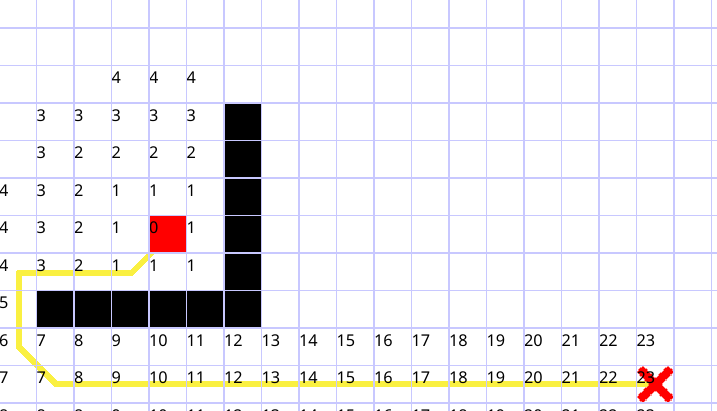
\includegraphics[width=1\linewidth]{astar-fail}
	\caption{$A^*$}
\end{subfigure}
\begin{subfigure}[b]{0.65\textwidth}
	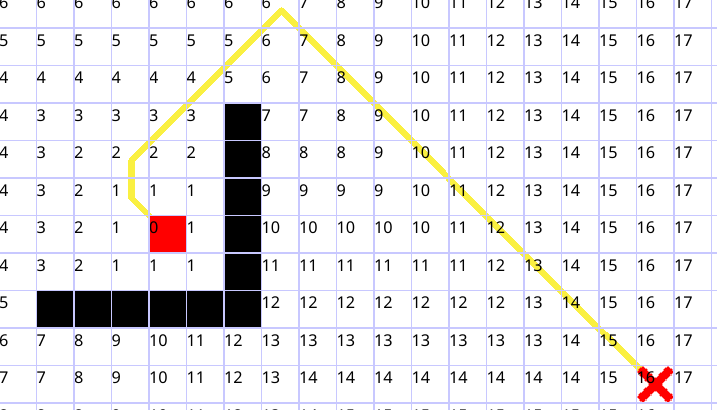
\includegraphics[width=1\linewidth]{astar-fail-dijkstra}
	\caption{Dijkstra}
\end{subfigure}
\caption{Pathfinding algorithms executed with diagonal movement allowed, and in the case of $A^*$, using the Manhattan distance as heuristic.}
\label{fig:counterexample:admissible}
\end{figure}

In figure \ref{fig:node-expansion} we can see a visual comparison of the number of nodes explored using algorithms \ref{alg:dijkstra}, \ref{alg:greedy} and \ref{alg:astar} in a single example. For algorithms \ref{alg:greedy} and \ref{alg:astar}, we have used the Manhattan distance as heuristic. We can see that Dijkstra explores many more nodes than the other two (it explores even more nodes that didn't fit in the image), while Greedy Best-First Search explores many fewer nodes but the path it finds isn't optimal, since the distance of the path it calculates is $35$, while Dijkstra and $A^*$ find paths of distance $33$.

\begin{figure}
\centering
\begin{subfigure}[b]{0.45\textwidth}
	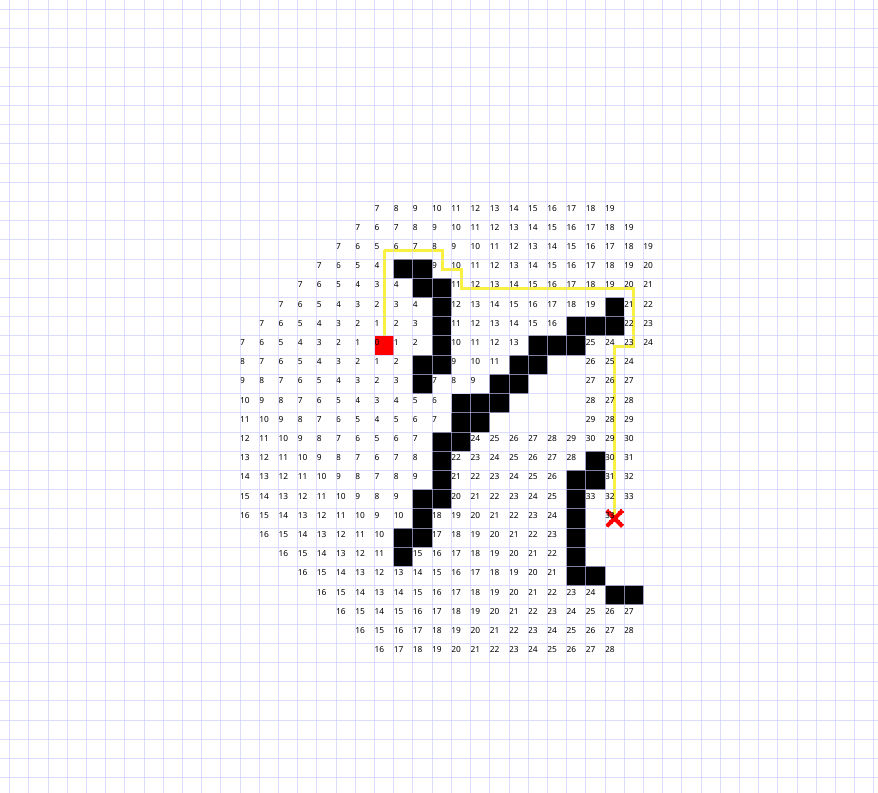
\includegraphics[width=1\linewidth]{astar-nodes}
	\caption{$A^*$}
\end{subfigure}
\begin{subfigure}[b]{0.45\textwidth}
	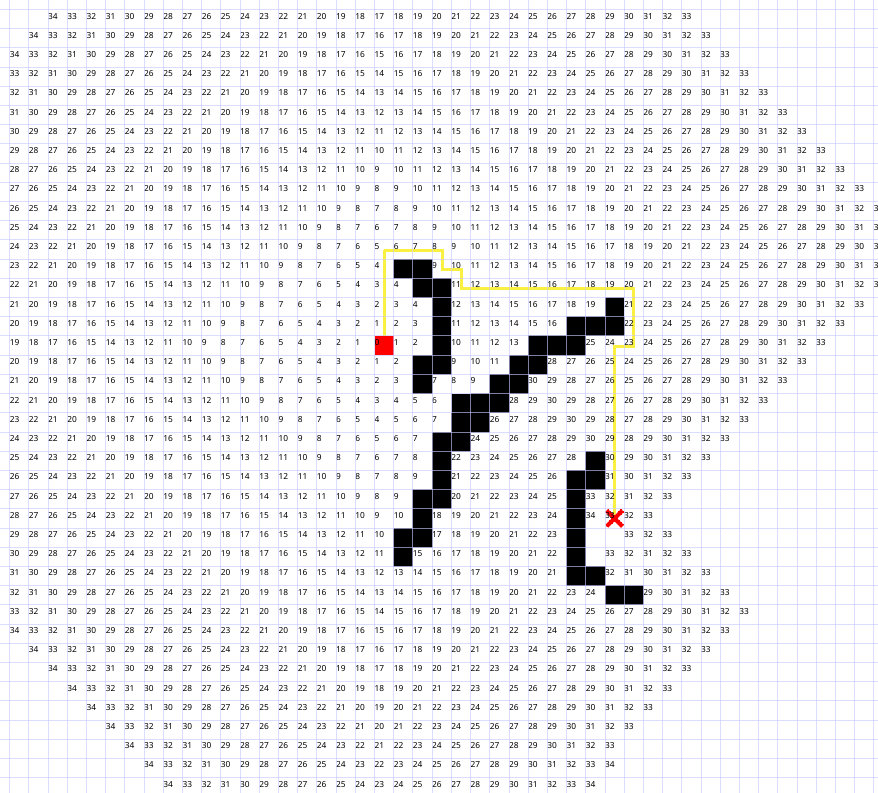
\includegraphics[width=1\linewidth]{dijkstra-nodes}
	\caption{Dijkstra}
\end{subfigure}
\begin{subfigure}[b]{0.45\textwidth}
	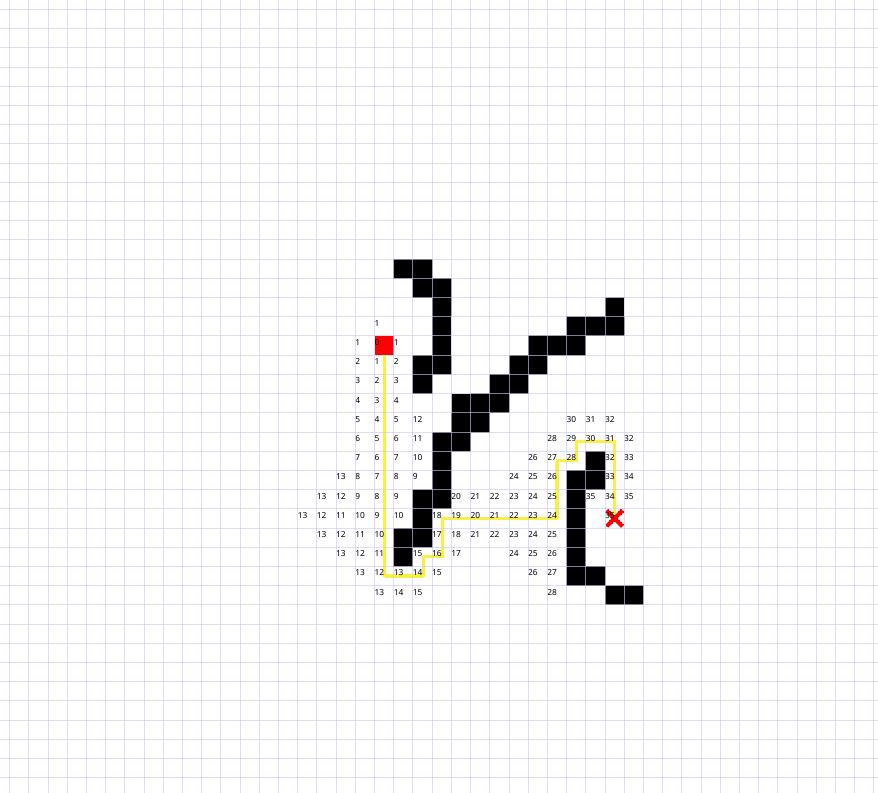
\includegraphics[width=1\linewidth]{greedy-nodes}
	\caption{Greedy Best-First Search}
\end{subfigure}
\caption{Pathfinding algorithms executed with diagonal movement allowed, and in the case of $A^*$, using the Manhattan distance as heuristic.}
\label{fig:node-expansion}
\end{figure}


\chapter{Heuristics}
In the previous chapter we have proved that as long as the heuristic is admissible, $A^*$ produces optimal paths. But not any admissible heuristic will give us the same performance. We've seen that by taking the admissible heuristic $h(u) = 0 \  \forall u \in V$, the algorithm becomes equivalent to Dijkstra, so we haven't gained anything.

$A^*$ is part of a class of algorithms, which we will call $\mathcal{A^*}$, and by selecting the g-score and h-score functions we select one of the algorithms from the class. We normally only change the h-score, and use the g-score defined previously, but notice how if we make $g(u) = 0 \  \forall u \in V$, then we get the Greedy Best-First Search algorithm seen in section \ref{section:greedy}. However, unless we explicitly say otherwise, we will always use the g-score we defined in section \ref{section:astar} for our $A^*$ algorithms.

The class $\mathcal{A^*}$ is a subclass of a larger set of algorithms which are usually known as \textbf{informed} or \textbf{heuristic search algorithms}.

In this chapter, we will see that there are heuristics which also make $A^*$ optimal, meaning that we can reduce the number of nodes expanded with respect to other algorithms of $\mathcal{A^*}$.

\section{Consistent heuristics}

\begin{definition}
A heuristic $h$ is said to be \textbf{consistent} or monotone if and only if, $\forall u, v \in V$,
\begin{equation}
	h(u) \leq \delta(u, v) + h(v)\label{eq:consistency}
\end{equation}
and
\begin{equation}
	h(t) = 0 \  \forall t \in T
\end{equation}
where $T$ is the set of goal nodes.
The relation shown in \ref{eq:consistency} is called the triangle inequality.
\end{definition}

For example the heuristic defined as $h(u) = 0 \  \forall u \in V$ is trivially consistent.

\begin{proposition}
\label{prop:consistent}
Given a heuristic $h$,
\[ h \text{ is consistent} \Rightarrow h \text{ is admissible} \]
\end{proposition}
\begin{proof}
Let $T$ be the set of goal nodes. We will prove that $\forall u \in V$ such that it has a connected preferred goal node in $T$, $h(u) \leq \hat{h}(u)$, by induction on the number of steps from $u$ to its preferred goal node in an optimal path $P$.

Let $t$ be a preferred goal node of $u$. If there are 0 steps from $u$ to $t$ in $P$, then $u = t$, and $h(u) = h(t) = 0 \leq \hat{h}(u) = 0$.

Now suppose that $u$ is $k > 0$ steps away from $t$ in $P$. Let $v$ be the successor of $u$ in $P$, which is $k-1$ steps away from $t$. Therefore, since $h$ is consistent,
\[ h(u) \leq \delta(u, v) + h(v) \]
But by our inductive hypothesis, $h(v) \leq \hat{h}(v)$, and therefore
\[ h(u) \leq \delta(u, v) + \hat{h}(v) = \hat{h}(u) \]
since $P$ is an optimal path.
\end{proof}

The converse is not true in general, although in practice it can be difficult to find an admissible heuristic that is not also consistent. We will show this with a counterexample. Take the graph from figure \ref{fig:heuristic}, and let $C$ be the single goal node. Let's define the heuristic as
\begin{align*}
h(A) &= 4\\
h(B) &= 1\\
h(C) &= 0
\end{align*}
The heuristic is clearly admissible, since $h(A) \leq \hat{h}(A) = 4$, $h(B) \leq \hat{h}(B) = 3$, and $h(C) \leq \hat{h}(C) = 0$. But it is not consistent, since $h(A) > \delta(A, B) + h(B) = 1 + 1 = 2$.

\begin{figure}
\centering
\begin{tikzpicture}
	[scale=.8, auto, node_style/.style={circle, draw=blue, fill=blue!20},
	edge_style/.style={draw=black, ultra thick}]
	\node[node_style] (n1) at (-5,0) {A};
  	\node[node_style] (n2) at (0,0) {B};
  	\node[node_style] (n3) at (5,0) {C};
  	
  	\draw[edge_style] (n1) edge node{1} (n2);
  	\draw[edge_style] (n2) edge node{3} (n3);
\end{tikzpicture}
\caption{A weighted undirected graph.}
\label{fig:heuristic}
\end{figure}

The following result is of special interest, since it will allow us to design $A^*$ algorithms which don't require to re-open already closed nodes, simplifying the implementation, and will be useful in our proof of optimality.

\begin{proposition}
\label{prop:closed-optimal}
With a consistent heuristic, any node $u$ closed by $A^*$ satisfies
\[ g(u) = \hat{g}(u) \]
\end{proposition}
\begin{proof}
Remember that our definition of the g-score implied $g(v) \geq \hat{g}(v) \ \forall v \in V$.

Consider the state just before closing a node $u$, and suppose $g(u) > \hat{g}(u)$. Since $u$ is about to be closed, it means it is connected to the source node $\alpha$, and therefore an optimal path $P$ exists between $\alpha$ and $u$. Since $g(u) > \hat{g}(u)$, the algorithm hasn't found $P$ or any other optimal path. Since it did not find $P$, by Lemma \ref{lemma:astar1},
\[ \exists v \in O \mid g(v) = \hat{g}(v) \]
and such that $v$ is part of $P$.

If $u = v$, then the proof is finished. Suppose $u \neq v$. Then, we have
\[ \hat{g}(u) = \hat{g}(v) + \delta(v, u) = g(v) + \delta(v, u) \]
since $P$ is an optimal path from $\alpha$ to $u$, and $v$ is part of $P$. Then, by our supposition,
\[ g(u) > g(v) + \delta(v, u) \]
Adding the $h(u)$ to both sides,
\[ g(u) + h(u) > g(v) + \delta(v, u) + h(u) \geq g(v) + h(v) \]
where in the second inequality we have used equation \ref{eq:consistency}.

Note that this result is equivalent to
\[ f(u) > f(v) \]
which contradicts the fact that $u$ was selected for expansion, when $v$ was available and should have been picked first by the algorithm.
\end{proof}

By our definition of the g-score, Proposition \ref{prop:closed-optimal} implies that when a node is closed, the algorithm has found an optimal path from the source node to the closed node. We can modify our $A^*$ code so that, when examining the neighbours of the node we are expanding, we check if the neighbour is already closed, and if it is, skip examining it again, like we did in Dijkstra. We will leave it to the reader to re-write the pseudocode with this new condition, but note that it is only valid if we use consistent heuristics.

The following result is also very strong, as it tells us that nodes are closed in a monotonic order of their score value.

\begin{lemma}
\label{lemma:order}
Consider the ordered set of the nodes closed by $A^*$, 
\[ \{ \alpha = n1, n2, \dots, n_m \} \]
ordered by the time they were closed by the algorithm. If the heuristic is consistent, then, for $p, q \in \{ 1, \dots, m \}$,
\[ p \leq q \Rightarrow f(n_p) \leq f(n_q) \]
\end{lemma}
\begin{proof}
Let $u$ be a closed node, and $v$ the node closed just before $u$. Suppose the optimal path $P$ computed by $A^*$ from the source node $\alpha$ to $u$ does not go through $v$. This means that the algorithm selected $v$ for expansion when $u$ was also available, which means $f(v) \leq f(u)$, proving the Lemma.

Now suppose that the optimal path to $u$, $P$, does go through $v$. Then, $\hat{g}(u) = \hat{g}(v) + \delta(v, u)$. By Proposition \ref{prop:closed-optimal}, we know that $g(u) = \hat{g}(u)$ and $g(v) = \hat{g}(v)$. Then,
\begin{align*}
f(u) &= g(u) + h(u)\\
&= \hat{g}(u) + h(u)\\
&= \hat{g}(v) + \delta(v, u) + h(u)\\
&\geq \hat{g}(v) + h(v)\\
&= g(v) + h(v) = f(v)
\end{align*}
where we have used equation \ref{eq:consistency}.

Since this is valid for any two nodes that are adjacent in the sequence, then we can clearly see by induction that
\[ p \leq q \Rightarrow f(n_p) \leq f(n_q) \]
\end{proof}


\section{Optimality of $A^*$}
Choosing consistent heuristics has a practical benefit. Like we've seen in Proposition \ref{prop:closed-optimal}, with a consistent heuristic we can avoid having to re-open nodes which were already closed. We will prove that with a consistent heuristic, $A^*$ is also optimal. By proposition \ref{prop:consistent} we see that consistency is a stronger condition than admissibility, and therefore by theorem \ref{thm:astar}, with a consistent heuristic the algorithm will still find optimal paths.

\begin{definition}
Given two admissible algorithms $A$ and $B$, we say that $A$ \textbf{dominates} $B$ if and only if the set of nodes expanded by $A$ is a subset of the set of nodes expanded by $B$.
\end{definition}

\begin{definition}
Given two admissible algorithms $A$ and $B$, we say that $A$ \textbf{strictly dominates} $B$ if and only if $A$ dominates $B$ and $B$ does not dominate $A$.
\end{definition}

\begin{definition}
Given a heuristic search algorithm $A$, we say that $A$ is \textbf{no more informed} than $A^*$ if $A$ has access to the same heuristic information as $A^*$, but placing no restriction in how it uses it, and does not have any extra information that $A^*$ does not have about unvisited nodes.
\end{definition}

We can then treat the heuristic as a parameter of the graph, where each node $u$ has an assigned value $h(u)$, and all heuristic search algorithms no more informed than $A^*$ have access to this information.

We will also assume that all the algorithms discussed use a sequential approach to expanding nodes, only expanding nodes that have previously been seen from another node, and starting the expansion on the source node $\alpha$.

\begin{lemma}
\label{lemma:astar-opt}
Suppose we have an admissible heuristic, and suppose that $A^*$ has not terminated yet. Then, for every closed node $u$,
\[ f(u) \leq f^* \]
\end{lemma}
\begin{proof}
If $T$ is the set of goal nodes, then $u \not \in T$ since the algorithm has not terminated. By Lemma \ref{lemma:astar2}, at the time time the node $u$ was closed, there existed a node $v \in O$ which is part of an optimal path $P$ from the source node $\alpha$ to a preferred goal node of $\alpha$ such that $f(v) \leq f^*$.
But since $u$ was closed before $v$, we have
\[ f(u) \leq f(v) \leq f^* \]
\end{proof}

\begin{proposition}
\label{prop:surely}
If the heuristic is consistent, then $A^*$ expands every node reachable from the source node $\alpha$ with optimal distance strictly bounded by $f^*$.
\end{proposition}
\begin{proof}
Let $t$ be the goal node at which $A^*$ terminates its execution. Since $A^*$ is admissible by hypothesis, then $f(t) = f^*$. Since by Lemma \ref{lemma:order} $A^*$ closes nodes in non-decreasing order of their score, there can't exist a non-closed node $u$ with $f(u) < f(t) = f^*$. Therefore, all such nodes must have been closed by the time the algorithm closes $t$, and by Proposition \ref{prop:closed-optimal}, the distance found by the algorithm from the source node is optimal. Then, for any closed node $u$ with score strictly less than $f^*$, $f(u) = g(u) + h(u) = \hat{g}(u) + h(u) < f^*$ which implies $\hat{g}(u) < f^*$.
\end{proof}

\begin{definition}
We say that every node expanded with the property from Proposition \ref{prop:surely} is \textbf{surely expanded} by $A^*$. Given a source node $\alpha$, we will write the set of nodes surely expanded by $A^*$, that is, with its optimal distance from the source strictly bounded by $f^*$, as $N_{f^*}$.
\end{definition}

\begin{theorem}[Optimality of $A^*$]
\label{thm:astar-optimality}
Let $A$ be an admissible algorithm no more informed than $A^*$, and let $h$ be a consistent heuristic used by the algorithms. Then, $A$ will always expand all nodes surely expanded by $A^*$.
\end{theorem}
\begin{proof}
Let $G = (V, E)$ be a graph, and $\alpha \in V$ the source node with which we will execute the algorithms, and $T$ the set of goal nodes. Let $u$ be a node surely expanded by $A^*$, that is, $u \in N_{f^*}$. Suppose $A$ also halts when expanding a node with cost $f^*$.

Suppose $A$ does not expand $u$. Now, consider a new graph $G' = (V', E')$ which we create by taking $G$, and adding a new goal node $t$ and an edge $e = (u, t)$ with cost $w(e) = h(u) + \Delta$ where
\[ \Delta = \frac{1}{2} (f^* - \max \{ f(v) \mid v \in N_{f^*} \}) > 0 \]
Then, $V' = V \cup \{ t 	\}$ and $E' = E \cup \{ e \}$.

In this new graph, we see that when $A^*$ expands $u$, it will assign $t$ with a score of
\[ f(t) = g(t) + h(t) = g(t) = g(u) + w(e) = f(u) + \Delta \leq f^* - \Delta < f^* \]
Therefore, there will be a new solution path with cost at most $f^* - \Delta$, which will be found by $A^*$.

We have to see that in this new graph $G'$, consistency is maintained. Since we left the h-score unchanged for the nodes in $G$, consistency still holds for any pair of values in $G$ by hypothesis. Then, we only have to check that consistency holds for any pair of values containing the added node $t$. Since $t$ is a goal node, $h(t) = 0$, and all we have to check is that $\forall v \in V \  h(v) \leq \delta(v, t)$.

Suppose that $\exists v \in V$ for which $h(v) > \delta(v, t)$. Then,
\[ h(v) > \delta(v, t) = \delta(v, u) + w(e) = \delta(v, u) + h(u) + \Delta \]
which violates the heuristic's consistency in $G$, since $\Delta > 0$.

Since $A$ is not more informed than $A^*$, it will behave the same way in $G'$ as it did in $G$, therefore not expanding $u$ and failing to find the path to $t$ with cost lower than $f^*$, which contradicts the fact that $A$ is admissible.
\end{proof}

\begin{definition}
A \textbf{tie-breaking} rule is the rule that $A^*$ uses to choose the next node to expand when there is more than one node with the same score.
\end{definition}

We observe that in cases in which there are no non-goal nodes with score $f^*$, the set of nodes surely expanded by $A^*$ is actually the entire set of nodes expanded by $A^*$. This happens when $h(u) < \hat{h}(u)$ for every node $u$ in the graph, and in this case we say that the algorithm is not fully informed \cite{optimality}. If there are nodes with score equal to $f^*$ other than the preferred goal node, the algorithm may potentially have to expand all the nodes with such score until it finds the preferred goal node. Then, the optimality of the algorithm depends on the tie-breaking rule used.

The following result is useful when we can't find consistent heuristics for some specific problems. It tells us that by finding higher bounds of an admissible heuristic, we generally can improve efficiency when there is a single goal node. This efficiency is, of course, bounded by that of a consistent heuristic, as we proved in Theorem \ref{thm:astar-optimality}.


\begin{theorem}
\label{thm:dominating-heuristic}
Let $G = (V, E)$ be a graph, let $h, h'$ be two admissible heuristics, and let $A^*_h, A^*_{h'} \in \mathcal{A^*}$ be the $A^*$ algorithms using these heuristics. Suppose we only have a single goal node $t$. Then,
\[ h'(u) \geq h(u) \  \forall u \in V \Rightarrow A^*_{h'} \text{ dominates } A^*_h \]
\end{theorem}
\begin{proof}
Suppose $A^*_h$ does not expand a node $u \in V$. Then, it suffices to show that $A^*_{h'}$ does not expand $u$ either.

If $u$ is not expanded by $A^*_h$, then either $f(u) > f(t)$ or $f(u) = f(t)$ and the tie-breaking rule selected $t$ before $u$. Let's call $f'$ the score used by $A^*_{h'}$.

Since $h'(u) \geq h(u)$, $f'(u) = g(u) + h'(u) \geq g(u) + h(u) = f(u)$. Then, if $f(u) > f(t)$, we have $f'(u) > f'(t)$ and $u$ will not be expanded. If $f(u) = f(t)$ and $h(u) = h'(u)$, then $f'(u) = f'(t)$, and the same tie-breaking rule will still select $t$ before $u$, therefore not expanding $u$.
\end{proof}

Suppose there was more than one goal node in the premises of Theorem \ref{thm:dominating-heuristic}. Let $t$ be the preferred goal node found by $A^*_h$, and $t'$ the one found by $A^*_{h'}$. Since both heuristics are admissible, and both $t$ and $t'$ are preferred goal nodes, $f(t) = \hat{g}(t) = \hat{g}(t') = f'(t')$. In the case where $f(u) = f(t)$ and $h(u) = h'(u)$, we would have $f'(u) = f'(t')$, but the tie-breaking rule could expand $u$ before $t'$, so the result would not hold in this case.

Note that, in general, it is very difficult to find a heuristic such that $h(u) = \hat{h}(u) \  \forall u \in V$, so we usually have to settle for some good lower bound by approximating this value.

\begin{theorem}
\label{thm:exact-heuristics-consistency}
Let $G = (V, E)$ be a graph, and consider a single goal node $t$. Then,
\[ h(u) = \hat{h}(u) \  \forall u \in V \Rightarrow h \text{ is consistent} \]
\end{theorem}
\begin{proof}
If $h = \hat{h}$, then $\forall u, v \in V$, we have $h(u) = \delta(u, t)$ and $h(v) = \delta(v, t)$.
The consistency equation immediately follows, since $\delta(u, t) \leq \delta(u, v) + \delta(v, t)$, the case of equality being when $v$ is part of an optimal path between $u$ and $t$.
\end{proof}

With non-consistent heuristics, the worst case complexity of $A^*$ becomes exponential, as it may potentially need to re-open each node several times \cite{martelli}. However, it is worth noting that in some cases inconsistent heuristics can actually more efficient, as it has been found to happen for the $A^*$ variant $\text{IDA}^*$ with the BPMX enhancement \cite{inconsistent}.

\section{Heuristics on grid graphs}
\label{section:heuristics-grid}
Our simulator uses a grid graph, so it is convenient to talk about some of the different heuristics we could use in this type of problem. In a grid graph, we have nodes uniquely identified by their coordinates, $(x, y)$, where $x,y \in \mathbb{Z}$.

\begin{definition}
\label{def:manhattan}
The \textbf{Manhattan distance} between two nodes with coordinates $(x_0, y_0)$ and $(x_1, y_1)$ is defined as
\begin{equation}
|x_1 - x_0| + |y_1 - y_0|
\end{equation}
\end{definition}

If the grid only allows horizontal and vertical movement, then it is easy to see that the Manhattan distance between any two nodes $u, v$ is actually $\delta(u, v)$. Therefore, a good heuristic in this case is to use the Manhattan distance from any node $u$ to the goal node, since in this case $h(u) = \hat{h}(u)$. By Theorem \ref{thm:exact-heuristics-consistency}, this heuristic will also be consistent.

\begin{definition}
The \textbf{Chebyshev distance} between two nodes with coordinates $(x_0, y_0)$ and $(x_1, y_1)$ is defined as
\begin{equation}
\max \{ |x_1 - x_0|, |y_1 - y_0| \}\label{eq:chebyshev}
\end{equation}
\end{definition}

If the grid allows diagonal movement, and moving diagonally has the same base cost as moving horizontally or vertically, then the Chebyshev distance between any two nodes $u, v$ is $\delta(u, v)$ and is also a consistent heuristic by Theorem \ref{thm:exact-heuristics-consistency}.

Remember that, as we saw in figure \ref{fig:counterexample:admissible}, the heuristic that uses the Manhattan distance is not admissible in a grid that allows diagonal movement, and as a result the algorithm will not be admissible.

\begin{definition}
The \textbf{octile distance} between two nodes with coordinates $(x_0, y_0)$ and $(x_1, y_1)$ is defined as
\begin{equation}
\max \{ |x_1 - x_0|, |y_1 - y_0| \} + \sqrt{2} \min \{ |x_1 - x_0|, |y_1 - y_0| \}\label{eq:octile}
\end{equation}
\end{definition}

The octile distance is a good heuristic when the base cost of moving diagonally is $\sqrt{2}$, using the Pythagorean theorem on the base costs of moving horizontally and vertically which would be $1$.

The Chebyshev and octile distances are actually special cases of a more general distance called the diagonal distance.

\begin{definition}
The \textbf{diagonal distance} between two nodes with coordinates $(x_0, y_0)$ and $(x_1, y_1)$ is defined as
\begin{equation}
D \max \{ |x_1 - x_0|, |y_1 - y_0| \} + (D' - D) \min \{ |x_1 - x_0|, |y_1 - y_0| \}\label{eq:diagonal-distance}
\end{equation}
where $D$ is the cost of moving horizontally and vertically, and $D'$ is the cost of moving diagonally.
\end{definition}

Observe that equation \ref{eq:chebyshev} is obtained by setting $D = D' = 1$ in equation \ref{eq:diagonal-distance}, and equation \ref{eq:octile} is obtained by setting $D = 1$ and $D' = \sqrt{2}$.

In all these cases, we could use the Euclidean distance between the points as heuristics, which is admissible, but the alternatives presented always dominate over it by Theorem \ref{thm:dominating-heuristic}.


\chapter{Pathfinding simulator}

In this brief chapter we will discuss the simulator built for this work, its options and implementation. As we already know, our simulator uses a grid graph. For the graphical interface, we have used the Qt library. The interface has a central widget where the grid graph is represented, and below it are some options to select the algorithm being used and its behaviour. There is also a menu bar from where we can do other things like save or load maps to a file.

In the grid, nodes are usually referred to as tiles. By left-clicking on a tile, we paint it with the currently selected weight or tile type. We have pre-defined some tile types (wall, floor, forest and water), and an option to create a custom tile type with a weight set by the user. The weight of the selected tile type is shown next to the tile type selection combo box. The weight of wall tiles is $\infty$, so painting a node with a tile type of wall is equivalent to 'removing' or disconnecting the node from the grid. We can think of painting a tile with some weight as setting the weights of the edges that go from adjacent tiles (neighbours) to that tile.

The algorithms implemented are the ones we have presented in chapter \ref{chapter:algorithms}, and the heuristics which are available for the algorithms that use one, namely $A^*$ and Greedy Best-First Search, are the ones presented in section \ref{section:heuristics-grid}.

The selected algorithm will execute itself interactively each time the grid changes, showing with a yellow path the path found by the algorithm from the source to the goal node, if it exists. This path will be an optimal path if and only if the algorithm used is admissible.

There is an option to show the cost to each of the nodes which the algorithm had examined by the time it terminated. This can be especially useful to get an idea of number and the position of the nodes that have been expanded in its execution, and the number in the goal tile will be the optimal distance from the source, as long as the algorithm is admissible.

We can drag and drop the source and goal tiles (represented with a red square and a red cross respectively) into any other tile with the right mouse button. Using the mouse wheel, we can zoom in and out on the map, and by dragging with the middle mouse button, we can pan the view.

There are also different tools or modes for painting tiles, introduced only for the sake of simplicity. With the pencil tool, we paint the tiles that are under the cursor. The bucket tool paints all tiles in an enclosed region where the weights are the same as the one where we click initially. The line tool allows to create approximations of lines by dragging with the left mouse button from an initial point to an end point, using Bresenham's algorithm \cite{bresenham}. Finally, the rectangle tool allows us to paint a filled rectangle by definind two opposing corners, using the left mouse button.

We can enable or disable diagonal movement with the simple click of a checkbox. We can also enable or disable corner movement, which means moving diagonally between two tiles when there is a wall tile which is adjacent to both tiles.

The simulator has the option to save the current map to a file, as well as to load a map from a file. The format used is a simple CSV file. The first line has two values, corresponding the width and height of the grid. The second line has four values. The first pair of values represents the coordinate of the top-left corner of the grid, $(x_0, y_0)$, and the second pair represents the coordinate of the bottom-right corner, $(x_1, y_1)$. The rest of the lines (which must equal the height in number), hold a certain number of values (which must equal the width in number) representing the weight of each tile.

Using this simple format means that we can also generate maps from another program using the same format, and then load them into the simulator. If the map used is smaller than the tiles the view can show, the tiles outside of the boundaries of the map are shown as walls.

\begin{figure}
\centering
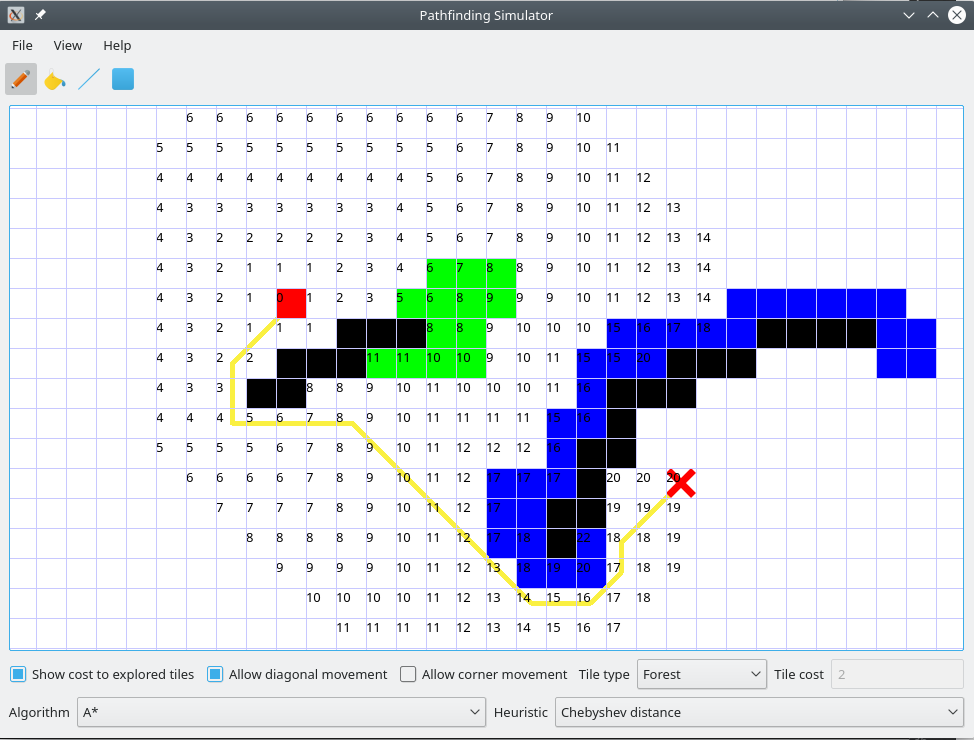
\includegraphics[width=1\linewidth]{pathfinding-simulator}
\caption{A screenshot showing the GUI of the pathfinding simulator. In this example, we are using the $A^*$ algorithm with the Chebyshev distance as heuristic, and with diagonal movement enabled. White tiles have cost 1, black tiles are walls (cost $\infty$), green tiles have cost 2 and blue tiles have cost 5.}
\label{fig:pathfinding-simulator}
\end{figure}


% Benchmark chapter
\chapter{Comparison of the algorithms}
The goal of this chapter is to perform an experiment to compare the memory and time efficiency of the algorithms presented in this work in a particular set of problems. To achieve this, two benchmarks were run, each using a different dataset with a particular type of graph. In the first benchmark, we used a grid graph, like the ones the simulator uses, but with randomized weights. In the second benchmark, we used a graph generated from the roads of Florida, where each node is an intersection and each edge is a road. In the next sections, we will describe in detail how each benchmark was prepared and its results.

\section{Grid graph benchmark}
For this benchmark, we generated a 1000x1000 grid graph in which the weight of each tile is picked randomly from a value in the set $\{ 1, 3, 5, 7, 9, \infty \}$ on creation, with equal probability. Remember that a weight of $\infty$ represents a wall, or equivalently, a disconnected node, in a grid graph. The grid graph used does not allow diagonal movement.

We then select a random pair of source and goal tiles, making sure none of them is a wall tile. Then, we execute each of the algorithms evaluated with the given source and goal tiles, and measure the number of nodes they expand and their total execution time, as well as the distances of the paths they find by the time they are finished. We count a node expansion whenever a node is closed, that is, taken out from the priority queue for further examination. If there does not exist a path from the source to the goal nodes that were selected, the result is discarded, a new set of source and goal nodes are generated and the algorithms are evaluated again. We ensured to only evaluate the algorithms when a path exists since in the case a path did not exist, all algorithms would expand all the nodes connected to the source and then terminate unsuccessfully, which does not bring any useful information to the efficiency comparison that we are trying to achieve. This whole process is repeated 1000 times.

We have evaluated four algorithms on this benchmark: Dijkstra's algorithm, $A^*$ using the Manhattan distance as heuristic, $A^*$ using the Euclidean distance as heuristic, and Greedy Best-First Search using the Manhattan distance as heuristic. Note that, as we saw in section \ref{section:heuristics-grid}, the Manhattan distance is a consistent heuristic in our problem. With Proposition \ref{prop:closed-optimal} it was seen that a simpler implementation was possible where no closed nodes would never be re-opened, as long as the heuristic is consistent. However, we still used the same implementation as described in \ref{alg:astar}. Since we did not use the simpler implementation, the algorithm in this case may have expanded more nodes in some of the test cases than it would have if we had used it, but to keep it more general and fair, it was decided to use the same algorithm that was presented earlier.

We have included Greedy Best-First search just for the sake of seeing how much faster it is than the other algorithms, but remember that it is not admissible. In the benchmark, Dijkstra's algorithm, as well as the two $A^*$ algorithms, always found the optimal distance between the source and goal nodes. This makes sense, since Dijkstra is always admissible, and in this problem both the Manhattan distance and the Euclidean distances are admissible. On the other hand, Greedy Best-First search never found an optimal path in all of the 1000 test cases that were executed for the benchmark.

The results of the benchmark are presented in Table \ref{table:grid-benchmark}. It is clear how the $A^*$ algorithms dominate over Dijkstra. Compared to Dijkstra, $A^*$ using the Manhattan distance evaluated $25.16\%$ less nodes, and was $31.4\%$ faster, showing a clear advantage in memory and speed. On the other hand, $A^*$ using the Euclidean distance also did very good memory-wise, expanding $21.8\%$ less nodes than Dijkstra, but time-wise the gain was not that substantial, being only $5.3\%$ faster, probably due to a badly implemented heuristic function which made it took longer than expected to compute.

\begin{center}
	\begin{tabular}{lcc}
	\label{table:grid-benchmark}
	Algorithm & Expanded nodes (total) & Time ($s$)  \\
	\hline
	Dijkstra & 427985668 & 1407.05 \\
	$A^*$ (Manhattan distance) & 320286310 & 964.59 \\
	$A^*$ (Euclidean distance) & 334885701 & 1332.23 \\
	Greedy Best-First Search & 804469 & 76.50 \\
	\end{tabular}
	\captionof{table}{Summary of the results from the grid graph benchmark.}
\end{center}


\section{Road graph benchmark}

For the second benchmark, we used a dataset from the 9th DIMACS Challenge\cite{dimacs}, in particular, the graph that contains the roads of the state of Florida in the US. The graph contains 1070376 nodes, and 2712798 edges, where each node represents an intersection and each edge a road.

Every node has a latitude and longitude associated given in microdegrees, which represent the geographical coordinates of the node. We use this information to build a weighted graph, giving each edge a weight equal to the great-circle distance computed using the haversine formula \cite{haversine}. We will also use this information for the heuristics we will be using.

Similar to the procedure of the first benchmark, we randomly select two nodes and execute each of the algorithms until it terminates, and we repeat this process for 1000 times. Like before, we evaluated 4 algorithms: Dijkstra's algorithm, $A^*$ with the Euclidean distance as heuristic, $A^*$ with the great-circle distance as heuristic, and Greedy Best-First Search with the Euclidean distance as heuristic. It is clear that both heuristics are admissible in this problem, but by Theorem \ref{thm:dominating-heuristic}, we expect the algorithm that uses the great-circle distance to dominate over the algorithm that uses the Euclidean distance.

The results of the benchmark are presented in Table \ref{table:road-benchmark}. Again, both $A^*$ algorithms clearly dominate over Dijkstra, and this time the difference was even more noticeable, due to the nature of the graph used. $A^*$ with the Euclidean distance expanded $68.3\%$ less nodes than Dijkstra, and was $71.2\%$ faster, while still finding optimal paths on all 1000 of the test cases. On the other hand, $A^*$ with the great-circle distance dominates over the other $A^*$ algorithm like we expected, expanding $253664$ less nodes, but the execution time is actually higher, taking $17.19 s$ more in total. This is because, even though the heuristic is more precise, and dominates the other one, it's actually more costly to compute, since the haversine formula involves trigonometric functions and their inverses, so the gain we get in memory, we lose in time efficiency. Still, the gain in memory is not that huge, because we are considering points which are relatively close to each other on the globe, where the Euclidean distance is a pretty good approximation of the great-circle distance. If we considered points further apart from each other, then there would probably be more noticeable differences, as the Euclidean distance would produce a poor estimate.

\begin{center}
	\begin{tabular}{lcc}
	\label{table:road-benchmark}
	Algorithm & Expanded nodes (total) & Time ($s$)  \\
	\hline
	Dijkstra & 580877763 & 1648.99 \\
	$A^*$ (Euclidean distance) & 184378253 & 474.59 \\
	$A^*$ (Great-circle distance) & 184124589 & 491.78 \\
	Greedy Best-First Search & 15077804 & 25.50 \\
	\end{tabular}
	\captionof{table}{Summary of the results from the road graph benchmark.}
\end{center}

Again, we included the Greedy Best-First Search algorithm just to see how fast it can find paths, even though they may not be optimal. This algorithm only found an optimal path 95 out of the 1000 test cases that were executed.

%
%\chapter{$A^*$ variants}
%
%In the last chapters we have mainly focused on the $A^*$ algorithm. But the addition rule used by the score, $f = g + h$, is not the only way to use the heuristic information we have, and we could also modify the way nodes are expanded, giving rise to new algorithms, fundamentally different from $A^*$, but still close enough to be considered part of the same family. In this chapter we will present some variants of the $A^*$ algorithm, explaining how they fundamentally change from the $A^*$ we have seen, and the benefits that using them may give us.
%
%
%\section{$IDA^*$}
%Iterative Deepening $A^*$, or $\bm{IDA^*}$, is a variant of $A^*$ based on iterative deepening search, which is a modification of Depth-First Search that finds the best depth limit. %TODO talk about DFS in the annex

%TODO jump-point searc, beam search, Theta*, D*...

%TODO make chapter on applications: 8-puzzle? route finding, AI, etc...


\chapter{Conclusions}
In this work, we have presented two algorithms which reliably find optimal paths in graphs as long as the necessary conditions are met, namely, 

Dijkstra's algorithm and $A^*$. Dijkstra's algorithm always finds optimal paths given any source node and set of goal nodes, but as it was reflected in our benchmark, it may potentially have to expand lots of nodes to find it. 

On the other hand, $A^*$ uses a heuristic to determine which nodes are more promising to explore next, by giving it a sense of the "direction" where the goal node is, which can avoid having to make many unnecessary node expansions in unpromising directions. But not any heuristic works. We have proved that in order for $A^*$ to reliably find optimal paths, the heuristic must be admissible, that is, it must never overestimate the real cost of an optimal path from a node to a preferred goal node. Moreover, we saw that if the heuristic is also consistent, then the algorithm becomes much more efficient, and avoids having to re-expand already expanded nodes. In general, we saw that higher lower bounds of the real optimal distances lead to better heuristics. On our benchmarks, $A^*$ clearly dominated over Dijkstra, even when the heuristic used, though still admissible, was not the best possible one.

As we saw in our roadmap benchmark, having a more precise heuristic is not always ideal. As we saw in Theorem \ref{thm:dominating-heuristic}, with a more precise heuristic, the algorithm will generally expand fewer nodes, which is true in our benchmark. However, due to the heuristic being more costly to compute, the time efficiency is actually worse than if we used a less precise heuristic which is faster to compute. This brings up a trade-off with which we have to deal when choosing an heuristic, and that is memory efficiency versus time efficiency. Finding the perfect balance between both is usually hard, so one has to choose depending on the specific priorities of the problem at hand.

We also briefly commented on the Greedy Best-First Search algorithm, which served us to present the concept of heuristics, but as we saw in our benchmarks, it fails to find optimal paths, as it is not designed for that. However, even if the path it finds is not optimal, it will always find a path if it exists, and given how much faster it is than the other algorithms, it could be a very good choice if all we need to do is prove if two nodes are connected, that is, checking if a path exists between two nodes.

There are many variants to the $A^*$ algorithm, but the core idea of doing an informed search based on a heuristic remains. No other algorithm that can reliably find optimal paths has been found which does better than $A^*$ in all cases, even after 50 years of its invention \cite{hart}, which explains why $A^*$ is still the de facto standard when it comes to pathfinding algorithms in many applications, like game development or robotics, and with the results compiled in this work, we can now understand why.

\begin{appendices}

\chapter{Data structures}

In this appendix we will briefly explain the data structures we used in our algorithms. We will only explain them on the interface level, and give the complexity of each of its operations. There are many different ways to implement these structures, but the details on the implementation and justification of the complexity are out of the scope of this work, but the information can be found in \emph{Introduction to Algorithms} by Thomas H. Cormen \textit{et al.}, or any other data structures or algorithmics book.

\section{Queue}
\label{annex:queue}
In algorithms \ref{alg:bfs} and \ref{alg:bfs_early_exit} we use a queue. A queue has two methods that modify the data in the structure:
\begin{itemize}
\item \emph{enqueue}: Adds an item at the back of the queue.
\item \emph{dequeue}: Removes the item in front of the queue. If there are no items in the queue, it does nothing.
\item \emph{empty}: Tells us whether the queue is empty or not.
\end{itemize}
For this reason, we say that a queue is a FIFO (first in, first out) structure, meaning that we will remove items from the queue in the same order as we inserted them. We always insert items from the back, and remove them from the front.

We also have a method, \emph{front}, which returns the item in the first position in the queue, but does not remove it.

All these methods have a time complexity of $O(1)$.

\section{Priority Queue}
\label{annex:priorityqueue}
In algorithms \ref{alg:dijkstra}, \ref{alg:greedy} and \ref{alg:astar} we use a priority queue. The priority queue works similarly to a queue, but each item also has a priority. This priority determines the order in which the items will be removed from the queue. In all our algorithms, we used a minimum priority queue, meaning that we associated a priority value to each item, and the item with minimum value would be served first. This is crucial for the correct functionality of all of our algorithms that use a priority queue. In Dijkstra, we used the current best distance to each node as the priority. In Greedy Best-First Search, we used the heuristic. And in $A^*$ we used the score function.

We use the following methods from the priority queue:
\begin{itemize}
\item \emph{insert}: Takes a pair of item and priority, and inserts the item into the right place in the priority queue. This method has a time complexity of $O(\log n)$ where $n$ is the number of elements in the priority queue.
\item \emph{removeMin}: Returns the item in the front of the priority queue, that is, the item with the smallest priority value (since it is a minimum priority queue), and removes it from the priority queue. This method has a time complexity of $O(1)$.
\item \emph{empty}: Tells us whether the queue is empty or not. Its complexity is $O(1)$.
\end{itemize}

We use the priority queue to get the node with minimum score (or distance in the case of Dijkstra, and h-score in the case of Greedy Best-First search) as the next node to be explored and closed. We also use this fact in many of the proofs.

Note that there are other implementations of the priority queue in which insertion is $O(1)$ and removing the item with minimum value is $O(\log n)$, but in the end it does not matter which one we use.

\section{Set}
A set is an unordered list of unique items, but differs in implementation from a regular array, since it is usually implemented using a hash map, so lookup is much faster. We use mainly two operations on the set: the \emph{add} method, which inserts an item into the set, and the \emph{lookup} method (which we represented using mathematical notation in our conditions), which determines whether an item is part of the set or not. Both of these operations have a time complexity of $O(1)$.

\section{Map}
A map is a structure that stores data in pairs of key and value. Once we have some data in it, we look up using a key, which retrieves its corresponding value. In all of our algorithms, we used maps to store the node we came from for each visited node. In Dijkstra and $A^*$, we also used maps to store the current best distance from the source to each node, or equivalently the g-score. A map has two main methods: one to insert data and one to look up data. We have represented this using square bracket notation:
\begin{itemize}
\item To insert or update data in a map $d$, we use $d[key] = value$. If the key did not exist in the map, it will be added with the given value. If the key already existed in the map, its value will be updated to the given value.
\item To look up data in a map $d$, we use $d[key]$, which would return the value associated to the given key. If the key was not in the map, this operation is illegal and the program should throw an error. In our case, we always initialize the maps at the beginning of the algorithms, so we can never run into this kind of problem.
\end{itemize}
Inserting and looking up data in a map has a time complexity of $O(1)$.

\end{appendices}


\begin{thebibliography}{99}

\bibitem{ai} S. Russell, P. Norvig, \textsl{Artificial Intelligence: A Modern Approach}, Third Edition, chapter 3, (2009)

\bibitem{dijkstra} E. W. Dijkstra, \textsl{A note on two problems in connexion with graphs}, Numerische Mathematik 1, pp. 269–271, (1959)

\bibitem{hart} P. E. Hart, N. J. Nilsson, and B. Raphael, \textsl{A formal basis for the heuristic determination of minimum cost paths}, (1968), IEEE Transactions of Systems Science and Cybernetics, SSC-4, 2

\bibitem{bellman-ford} Jørgen Bang-Jensen, Gregory Gutin, \textsl{Digraphs: Theory, Algorithms and Applications}, (2000)

\bibitem{optimality} R. Dechter, J. Pearl, \textsl{Generalized Best-First Search Strategies and the Optimality of A*}, Journal of the ACM, 32(3), pp. 505-536, (1985)

\bibitem{martelli} A. Martelli, \textsl{On the complexity of admissible search algorithms}, Artificial Intelligence 8, pp. 1–13, (1977)

\bibitem{inconsistent} N. R. Sturtevant, Z. Zhang, R. Holte, J. Schaeffer, \textsl{Using Inconsistent Heuristics on A* Search}, University of Alberta, Department of Computer Science

\bibitem{dimacs} 9th DIMACS Implementation Challenge,\\
\url{http://www.dis.uniroma1.it/challenge9/}

\bibitem{bresenham} J. E. Bresenham, "Algorithm for computer control of a digital plotter", \textsl{IBM Systems Journal}, 4(1), pp. 25-30, (1965)

\bibitem{haversine} José de Mendoza y Ríos, "Memoria sobre algunos metodos nuevos de calcular la longitud por las distancias lunares y explicaciones prácticas de una teoría para la solución de otros problemas de navegación", (1795)

\end{thebibliography}

\end{document}
